\graphicspath{{Figures/}}
\chapter{Instable Feedback QP Control for Kinematic-Controlled Robots} \label{chap:instable qp}
In the previous chapter, we proposed a general formulation for the kinematic constraints \eqref{eq:second order ODI distance}--\eqref{eq:second order ODI vel} based on an adaptive-gains method.  
The conducted experiments on HRP-4 humanoid robot in closed-loop showed the performance of the proposed approach over the state-of-the-art methods. 
However, the observation of oscillations at the constraints boundary  when the constraint gains raises some questions about the stability and robustness of our formulation. For instance, oscillations are noticed at the CoM constraint boundary in  \cref{fig:CoM evolution} and which we have argued to be due to the non-modeled flexibilities at the ankles. Damped oscillations are also observed at the collision-avoidance constraint boundary in \cref{fig:different-initial-condition} and seem to correlate with high constraint gains. This fact implies that choosing high task gains will produce similar behaviors as well. These oscillations are not the desired behavior as they are generally referred to as a sign of instability. In practice, it results in discontinuous and jerky motion that can be unsafe for the robot (structural damage, actuator wearing) and the operators surrounding it. This motivates us in this chapter to investigate the sources of instability of the closed-loop QP control system.

To start our reasoning, one important remark is that the robot used for experiments is a \emph{‘kinematic-controlled robot’}, i.e., torque-controlled robots equipped with high-gains joint controllers that compute the desired joint torques $\desTau$ for the actuators (see \cref{fig:position controller}). These joint-controllers are designed by the manufacturer to track the desired joint position or velocity. Hence, if the robot behavior is instable, it means that the joint-controllers are tracking an unbounded desired input.   Since these desired inputs (joint-position or velocity) result from the double integration of the QP output $\genDesConfDDot$, it means that the QP controller generated solutions are not stable. 

%Several research works have reported similar instability phenomena of relative severity (e.g., strong sustained oscillations), see e.g.,~\cite{feng2015journalOfFieldRobotics,johnson2015journalOfFieldRobotics,dedonato2017frontiers,koolen2016ijhr}. Interestingly, it has been noted in~\cite{feng2015journalOfFieldRobotics} that the oscillations and undesired behaviors are related to the double integration of the QP output $\desConfDDot$. However, no further investigation was made to elucidate the cause. Instead, only workaround solutions have been proposed to bypass this issue. 
%Moreover,  the robots used in the above cited works rely also on joint-controllers in addition to a feedforward torque term (\cref{fig:leaky integrator QP}). The only difference with robots in \cref{fig:position controller} is the joint-controllers are numerically-implemented, whereas  they are hardware-implemented  for kinematic-controlled robots. 
 
%In~\cite{feng2015journalOfFieldRobotics}, it has been noted that the oscillations and undesired behaviors are related to the double integration of the QP output $\desConfDDot$. However, no further investigation was made to elucidate the cause.
%Furthermore, we
%Despite our method is based on an analytical solution without considering the presence of non-modeled dynamics,  However, the robustness of our formulation is questioned especially when damped oscillations  have been observed at the constraint boundary for the collision avoidance (\cref{fig:different-initial-condition}) and CoM (\cref{fig:CoM evolution}) constraints. In addition, these non-robustness behaviors may appear at the tasks as well. 

%This motivates us in this chapter to not only study the robustness of our kinematic constraints formulation, but the tasks formulation robustness as well against non-modeled dynamics. A nonrobust closed-loop control scheme leads to instability which manifests as strong oscillations and jerky motion which can be unsafe for the robot (structural damage, actuator wearing), and the people surrounding the robot.   
%\begin{figure}
%	\centering
%	\begin{tikzpicture}[auto, node distance=2cm,>=latex']
%		\node [input, name=rinput] (rinput) {};
%		\node [block, right of=u, node distance = 2.0 cm](joint controller) {Joint Controllers};
%		\node [tmp, below of= joint controller, node distance = 0.7 cm] (tmp){};
%		\node [block, right of=joint controller, node distance = 6 cm](robot) {Torque-Controlled Robot};
%		\node [tmp, right of= robot, node distance = 3.8 cm] (tmp2){};
%		\node [dotted_block, fit = (joint controller) (robot) (robot) (tmp)] (pos controller) {};		
%		\node at (pos controller.north) [above, inner sep=1.5mm] {Kinematic-Controlled Robot};
%		%	\draw [->] (u) -- node{$\jointCrtlIn$}(xd dynamics);
%		\draw [->] (rinput) -- node[pos=0.3]{$
%			\left[\desConf \ \desConfDot\right]
%			$}(joint controller);%node{$\desConfDDot$}(InvDyn);
%		%\draw [->] (QP.north) |- node{$\desConfDDot$}(integrator.west);
%		\draw [->] (joint controller) -- node{$\desTau$}(robot);
%		\draw [->] (robot) -- node[pos=0.65]{$
%			\left[\actConf \  \actConfDot\right]
%			$}(tmp2);
%		\draw [-] ([xshift=-35pt]tmp2) |- (tmp);
%		\draw [->] (tmp) -- (joint controller.south);
%		%	 			\draw [->] (sum) -- node{}(robot);
%		%	 			\draw [->] (integrator.east) -- node{$
%			%	 				\left[\desConf \ \desConfDot\right]
%			%	 				$}(feedback.west);
%		%	 			\draw [-] (robot) -- node{$
%			%	 				\left[\actConf \  \actConfDot\right]
%			%	 				$}(x2);
%		%	 			\draw [-] (x2) |- (aux);
%		%	 			\draw [->] (x2) -- (x3);
%		%	 			\draw [->] (aux) -- node{}(QP.south);
%		%	 			%	\draw [->] (alphad2) -- node{}([xshift=-10pt]InvDyn.south);
%		%	 			\draw [->] (alphad) -- node{}([xshift=-0pt]InvDyn.south);
%		%	 			%	\draw [-] (xd) |- node{}(alphad3);
%		%	 			%	\draw [->] (alphad3) -- node{}([xshift=10pt]integrator.south);
%		%	 			\draw [-] (x2) |- (xBis);
%		%	 			\draw [->] (xBis) -- (integrator.north);
%		%	 			\draw [-] (feedback.south) -- (sumTmp);
%		%	 			\draw [->] (sumTmp) -| (sum.north);
%		%	 			\draw [->] ([xshift=2pt]alphaD) |-  (integrator.west);
%		%	\draw [->] (alphaD) |- node{$\desConfDDot$}(integrator.west);
%		%	\draw [->] (disturbance) --node{$\jointDisturbIn$} (x dynamics.north);
%	\end{tikzpicture}		
%	\caption{Illustrative block scheme of a kinematic-controlled robot (dotted) which, for a matter of space, denotes ‘Robot’ block in \cref{fig:QP scheme for kinematic-control robots}-\ref{fig:whole control scheme}.}
%	\label{fig:position controller}
%\end{figure}

In this chapter, we  study the effect of the joint-controllers on the stability of the closed-loop system containing a QP controller and kinematic-controlled robot. Instead of considering the robot as a multi-DoF system, we only focus on a case-study:  1-DoF  system (an actuator servoed by a PD-controller). In \cref{sec-chap2:1-DoF robot}, we  introduce more in detail the kinematic-controlled robots and explain why the 1-DoF case-study is sufficient for the stability study. Then, we  model the dynamics of a DC motor servoed with a PD-controller. In \cref{sec-chap2:QP stability investigation}, we investigate the stability of a QP controller in cascade with the 1-DoF system following two closed-loop control schemes (\cref{fig:QP scheme for kinematic-control robots}), and show the pros and cons of each. Finally, we propose an approach that ensures the stability while reactively counterbalancing external disturbances.    
%Although it is a simple case but it is sufficient to understand 

%In our study, we will focus particularly on ‘kinematic-controlled robots’ which is a general term that encompasses the robots that are controlled by sending either the desired joint position (position-controlled) or the desired joint velocity (velocity-controlled). These robots are equipped with high-gains joint controllers that compute the desired joint torques $\desTau$ for the actuators (see \cref{fig:position controller}). Stiff kinematic-controlled robots are widely used in robotics and automation industry as the knowledge of the robot's dynamics is not required~\cite{garcia2004iros,rossi2014iros,zanchettin2017elsevier,singletary2022csl,polverini2017ral,suarez2018sciRob,lim2016journalOfFieldRobotics}. Nevertheless, their joint dynamics (joint controllers + actuators) are generally not known as they depend on the joint controller gains (fixed by the manufacturer not intended to be modified by the operator in almost all robots) and the actuators electro-mechanical constants. Consequently, the non-modeled joint-dynamics rise as the main factor of non-robustness of the closed-loop QP controller. Other non-modeled dynamics can be considered like sensor noises, and flexibilities especially for humanoid robots which often contains soft materials at the ankles to lower the walking impacts on the whole structure.  

%In this chapter, we will consider a simple example of a 1-DoF position-controlled robot controlled by a QP. This simple case-study will enables us to provide answers for the following questions (i) what leads the closed-loop QP control scheme to be non-robust and thereby instable; (ii) how can we ensure robustness of the closed-loop QP control. 
%First we will 


%\begin{itemize}
%	%	\item The gains adaptation method is based on an analytical solution without considering the presence of non-modeled dynamics
%	%	\item In the next section, we will particularly  focus on the case of kinematically controlled (position-controlled) robots which joint-dynamics is not modeled in addition to other factors like flexibilities and sensor noise 
%	%\item {\color{red} Since the analytical solution cannot be used anymore, we propose a robust constraint formulation based on Control Barrier Function theory }
%\end{itemize} 
%\section{State-of-the-Art}\label{sec-chap2:sota chap2}
%%QP control has been successfully applied to complex robots and scenarios~\cite{escande2014ijrr,salini2011icra,herzog2016autonomousRobot,kuindersma2016autonomousRobot,feng2014humanoids,nava2020ral,hamed2020ral,englsberger2015tro,klemm2020ral,basso2020ifac,reher2021arxiv-tro}. 
%%Yet, 
%Several research works reported instability phenomena of relative severity (e.g., strong sustained oscillations), see e.g.,~\cite{feng2015journalOfFieldRobotics,johnson2015journalOfFieldRobotics,dedonato2017frontiers,koolen2016ijhr}. Interestingly, the common factor in each reported shortcoming is that the joint torque control relies on joint-position and/or velocity feedback terms in addition to $\desTau$ (\cref{fig:leaky integrator QP}). In~\cite{feng2015journalOfFieldRobotics}, it has been noted that the oscillations and undesired behaviors are related to the double integration of the QP output $\desConfDDot$. However, no further investigation was made to elucidate the cause.
%
%Workaround solutions have been proposed to mitigate this issue. These palliative methods can be sorted into two categories: (i) \emph{low-level approaches} that act at the joint-level to prevent $\desConfDDot$ double integration from diverging; typically by implementing a leaky integrator~\cite{hopkins2015icra}; and (ii) \emph{high-level approaches}  where the QP formulation is substantially modified at the expense of a complex control-architecture~\cite{feng2014humanoids,feng2015journalOfFieldRobotics}, or by accounting for the joint feedback terms in the QP to adapt their gains~\cite{lee2022frontiersRobS} or for constraints feasibility concerns~\cite{cisneros2018iros}. Other approaches reported that lowering the task gains helps mitigating the instability~\cite{koolen2016ijhr,johnson2015journalOfFieldRobotics} which highlights the fact that task gains are also an interfering factor. Similar observation is made in~\cite{djeha2020ral,singletary2022csl} concerning the gains of the safety-constraint formulation. 
%
%The closed-loop task-space QP controller combined with a joint low-level kinematic-controlled robot,~\cref{fig:QP scheme for kinematic-control robots}\subref{subfig:feedback QP}, is also prone to previously described instability shortcomings.  
%The latter have been unnoticed in some control implementations that operate in feedforward (\cref{fig:QP scheme for kinematic-control robots}\subref{subfig:feedforward QP}). This leads to a decoupled control (similar to~\cite{feng2015journalOfFieldRobotics}), delegating the control accuracy to the joint controllers~\cite{bouyarmane2018tac,zanchettin2017elsevier,polverini2017iros_a}. In such cases, frequent initializations of the controller are needed to lower the discrepancy between real and control-model states due to non-modeled flexibilities or external disturbance. 

%\begin{figure}%[t!]
%	\centering
%	\begin{tikzpicture}[auto, node distance=2cm,>=latex']
%		\node [input, name=rinput] (rinput) {};
%		\node [tmp, right of=rinput, node distance = 0.0 cm](u){};
%		\node [block, right of=u, node distance = 0 cm](QP) {QP};
%		\node [tmp, right of=QP, node distance = 1cm] (alphaD){};
%		
%		%	\node [tmp, above of=InvDyn, node distance = 1. cm] (tmp1){};
%		\node [block, right of = QP, node distance = 3 cm] (integrator) {Double Integrator};
%		\node [sum, right of = integrator, node distance = 3.5 cm] (sum2){};
%		%			 			\node [block, left of = tmp1, node distance = 0.0 cm,xshift=-2pt] (integrator) {Leaky Integrator};
%		\node [block, right of = sum2, node distance = 2.2 cm] (feedback) {Joint Controllers};
%		
%		\node [tmp, below of=sum2, node distance = 1 cm] (xFeedback){};
%		\node [tmp, below of=QP, node distance = 1.0 cm] (xQP){};
%		\node [sum, right of = feedback, node distance = 2.2 cm] (sum){};
%		\node [tmp, above of=sum, node distance = 1.1 cm](InvDyn) {};
%		\node [block, right of=sum, node distance = 1.2 cm](robot) {Robot};		
%		\node [tmp, right of=robot, node distance = 0.8 cm](x){};
%		\node [tmp, right of=x, node distance = 0.7 cm](x2){};
%		
%		
%		%	\draw [->] (u) -- node{$\jointCrtlIn$}(xd dynamics);
%		
%		\draw [-] ([yshift=0pt]QP.north) |- node[above,pos=0.54]{$\desTau$}(InvDyn);
%		%\draw [->] (QP.north) |- node{$\desConfDDot$}(integrator.west);
%		\draw [->] (InvDyn) -- node[above,pos=0.9]{}(sum);
%		%		\draw [-] ([yshift=+2.5pt]QP.east) -| node[above,pos=0.3]{}([xshift=-50pt,yshift=2.5pt]InvDyn);
%		%		\draw [-] ([yshift=+2.5pt]QP.east) -| node[above,pos=0.3]{}([xshift=-50pt,yshift=2.5pt]InvDyn);
%		%		\draw [->] ([xshift=-50pt,yshift=2.5pt]InvDyn) |- node[above,pos=0.7]{$\desConfDDot$}(integrator.west);
%		\draw [->] (QP.east) |- node[above, pos = 0.8]{$\genDesConfDDot$}(integrator.west);
%		\draw [->] (sum) -- node{}(robot);
%		\draw [->] (integrator.east) -- node[above, pos = 0.5]{$
%			\left[\desConf \ \desConfDot\right]
%			$}(sum2);
%		\draw [->] (sum2.east) -- node{}(feedback);
%		\draw [->] (feedback.east) -- node{}(sum);
%		\draw [-] (robot) -- node[above, pos = 1]{$
%			\left[\actConf \  \actConfDot\right]
%			$}(x2);
%		\draw [-] ([xshift = 0pt]x2) |- (xFeedback);
%		\draw [->] (xFeedback) -- node[pos = 0.8]{$-$}(sum2);
%		%	\draw [->] (x2) -- (x3);
%		\draw [-] (xFeedback) -- node{}(xQP);
%		\draw [->] (xQP) -- node{}(QP);
%		%	\draw [->] (alphad2) -- node{}([xshift=-10pt]InvDyn.south);
%		%\draw [->] (alphad) -- node{}([xshift=-0pt]InvDyn.south);
%		%	\draw [-] (xd) |- node{}(alphad3);
%		%	\draw [->] (alphad3) -- node{}([xshift=10pt]integrator.south);
%		%	\draw [-] (x2) |- (xBis);
%		%	\draw [->] ([xshift = 4pt]x2) |- (feedback.east);
%		%			 			\draw [-] (xBis) -- (xBisInt);
%		%			 			\draw [->] (xBisInt) -- (integrator.north);
%		%	\draw [-] (feedback.south) -- (sumTmp);
%		%\draw [->] (sumTmp) -| node[pos=1, above, xshift =-5pt]{$+$}(sum.north);
%		
%		%	\draw [->] ([xshift=2pt]alphaD) |-  (integrator.west);
%		%	\draw [->] ([yshift=5pt]QP.east) |- (integrator.west);
%		%	\draw [->] (alphaD) |- node{$\desConfDDot$}(integrator.west);
%		%	\draw [->] (disturbance) --node{$\jointDisturbIn$} (x dynamics.north);
%	\end{tikzpicture}
%	
%	\caption{QP control scheme for torque-controlled robots with additional joint feedback. ‘Robot’ is torque-controlled.}
%	\label{fig:leaky integrator QP}
%\end{figure}
\begin{figure}[t!]
	\centering
	\subfloat[]{
		\begin{tikzpicture}[auto, node distance=2cm,>=latex']
			\node [input, name=rinput] (rinput) {};
			\node [tmp, right of=rinput, node distance = 0.5 cm](u){};
			\node [block, right of=u, node distance = 0 cm](QP) {QP};
			\node [tmp, right of=QP, node distance = 0.5 cm] (alphaD){};
			\node [block, right of=alphaD, node distance = 3 cm](integrator) {Double Integrator};
			\node [tmp, right of=integrator, node distance = 2.2 cm] (xd){};
			\node [block, right of=xd, node distance = 2 cm](robot) {Robot};
			\node [tmp, right of=robot, node distance = 1 cm](x){};
			\node [tmp, right of=x, node distance = 0.7 cm](x2){};
			\node [tmp, below of = QP, node distance = 0.7cm] (aux){};
			%	\draw [->] (u) -- node{$\jointCrtlIn$}(xd dynamics);
			\draw [->] (QP) -- node{$\desConfDDot$}(integrator);
			\draw [->] (integrator) -- node{$
				\left[\desConf \ \desConfDot\right]
				$}(robot);
			\draw [->] (robot) -- node{$
				\left[\actConf \  \actConfDot\right]
				$}(x2);
			\draw [-] (x) |- (aux);
			\draw [->] (aux) -- node{}(QP.south);	
			%	\draw [->] (disturbance) --node{$\jointDisturbIn$} (x dynamics.north);
		\end{tikzpicture}
		\label{subfig:feedback QP}}
	\hfil
	\subfloat[]{
		\begin{tikzpicture}[auto, node distance=2cm,>=latex']
			\node [input, name=rinput] (rinput) {};
			\node [tmp, right of=rinput, node distance = 0.5 cm](u){};
			\node [block, right of=u, node distance = 0 cm](QP) {QP};
			\node [tmp, right of=QP, node distance = 0.5 cm] (alphaD){};
			\node [block, right of=alphaD, node distance = 3 cm](integrator) {Double Integrator};
			\node [tmp, right of=integrator, node distance = 2.2 cm] (xd){};
			\node [block, right of=xd, node distance = 2 cm](robot) {Robot};
			\node [tmp, right of=robot, node distance = 1 cm](x) {};
			\node [tmp, right of=x, node distance = 0.7 cm](x2){};
			%	\node [tmp, right of=robt, node distance = 2 cm](x){};
			\node [tmp, below of = QP, node distance = 0.7cm] (aux){};
			%	\draw [->] (u) -- node{$\jointCrtlIn$}(xd dynamics);
			\draw [->] (QP) -- node{$\desConfDDot$}(integrator);
			\draw [->] (integrator) -- node{$
				\left[\desConf \  \desConfDot\right]
				$}(robot);
			\draw [-] (xd) |- (aux);
			\draw [->] (aux) -- node{}(QP.south);
			\draw [->] (robot) -- node{$
				\left[\actConf \  \actConfDot\right]
				$}(x2);
			%	\draw [->] (disturbance) --node{$\jointDisturbIn$} (x dynamics.north);
		\end{tikzpicture}
		\label{subfig:feedforward QP}}
%	\hfil
%	\subfloat[]{
%		\begin{tikzpicture}[auto, node distance=2cm,>=latex']
%			%	 			\node [input, name=rinput] (rinput) {};
%			%	 			\node [tmp, right of=rinput, node distance = 0.5 cm](u){};
%			\node [block, draw = black, ](QP) {QP};
%			\node [tmp, right of=QP, node distance = 0.5 cm] (alphaD){};
%			\node [block, right of=alphaD, node distance = 3 cm, draw = black, ](integrator) {Double Integrator};
%			\node [tmp, right of=integrator, node distance = 2.2 cm] (xd){};
%			\node [block, right of=xd, node distance = 2 cm, draw = black, ](robot) {Robot};
%			\node [tmp, right of=robot, node distance = 1 cm](x){};
%			\node [tmp, right of=x, node distance = 0.7 cm](x2){};
%			\node [tmp, below of = QP, node distance = 0.7cm] (aux){};
%			\node [tmp, below of = QP, node distance = 0.57cm] (aux2){};
%			%	\draw [->] (u) -- node{$\jointCrtlIn$}(xd dynamics);
%			\draw [->, color=black, ] (QP) -- node{$\desConfDDot$}(integrator);
%			\draw [->, color=black, ] (integrator) -- node{$
%				\left[\desConf \  \desConfDot\right]
%				$}(robot);
%			\draw [->, color=black, ] (robot) -- node{$
%				\left[\actConf \  \actConfDot\right]
%				$}(x2);
%			\draw [-, color=black, ] (x) |- ([xshift=-5pt]aux);
%			\draw [-, color=black, ] (xd) |- ([xshift=5pt]aux2);
%			%\draw [-] (aux) -- node{}(rinput);	
%			\draw [->, color=black, ] ([xshift=-5pt]aux) -- node{}([xshift=-5pt]QP.south);
%			\draw [->, color=black, ] ([xshift=5pt]aux2) --([xshift=5pt]QP.south);
%			%	\draw [->] (disturbance) --node{$\jointDisturbIn$} (x dynamics.north);
%		\end{tikzpicture}
%		\label{subfig:our QP}}		
	\caption{Different closed-loop QP control schemes for kinematic-controlled robots.
		%~\subref{subfig:leaky integrator QP} Leaky integrator QP in~\cite{hopkins2015icra}.
		~\subref{subfig:feedback QP} Feedback QP.
		~\subref{subfig:feedforward QP} Feedforward QP.}
		%~\subref{subfig:our QP} Proposed robust QP. }
	\label{fig:QP scheme for kinematic-control robots}
\end{figure}


\section{Kinematically-Controlled Robots}\label{sec-chap2:1-DoF robot}
\begin{figure}
	\centering	
	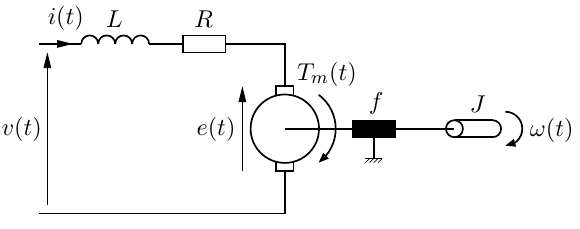
\includegraphics[width=0.6\columnwidth]{DCC model.pdf}
	\caption{DC motor model}
	\label{fig:DCmodel}
\end{figure}
\begin{table}
	\centering
	\begin{tabular}{|c|c|}
		\hline 
		& Parameters \\
		\hline
		Electrical & 
		\begin{tabular}{@{}c@{}}
			$v(t)$: Voltage input (V) \\
			$i(t)$: Current (A) \\ 
			$e(t)$: Electro-Motive Force (EMF) (V) \\
			$\tau_{\rm l}(t)$: Load torque (Nm) \\
			$\tau_{\rm m}(t)$: Motor torque (Nm) \\
			$L$: Inductance (H) \\ 
			$R$: Resistance ($\varOmega$) \\ 
			$K$: Torque and EMF constant (V.s.rad$^{-1}$)
		\end{tabular}\\
		\hline
		Mechanical & 
		\begin{tabular}{@{}c@{}}
			$\omega_m(t)$: Motor-side angular velocity\\
			$\omega(t)$: Link-side angular velocity\\
			$J$: Rotor inertia ($Kg.m^2$) \\ 
			$f$: Friction coef. ($N.m.s.rad^{-1}$) \\ 
			$N$: Gear ratio\end{tabular} \\
		\hline
	\end{tabular}
	\caption{Specification of the electrical and mechanical parameters.}
	\label{tab:DC motor paramters}
\end{table}
Stiff kinematic-controlled robots are widely used in robotics and automation industry as the knowledge of the robot's dynamics is not required~\cite{garcia2004iros,rossi2014iros,zanchettin2017elsevier,singletary2022csl,polverini2017ral,suarez2018sciRob,lim2016journalOfFieldRobotics,singletary2022csl}. Controlling a kinematic-controlled robot rely on a simple control strategy which consists in considering the robot with $n$-actuated DoF as a system of $n$ independent joints. Each joint is actuated with a motor servoed by a joint-controller, resulting in a Single-Input/Single-Output (SISO) system. The joint-level servoing can performed either in position (i.e., regulate the error between the desired joint position $\desConf$ and the actual joint position $\actConf$ to zero) or in velocity (i.e., regulate the error between the desired joint velocity $\desConfDot$ and the actual joint velocity $\actConfDot$ to zero)~\cite{albu-schaffer2007industrialRobot,albu-shaffer2007ijrr,mistry2008humanoids,iskandar2020iros,lim2016journalOfFieldRobotics,lim2017journalOfFieldRobotics}. %(\cref{fig:position controller}). 

The most known and documented joint-controller is the position Proportional-Derivative (PD) joint-controller~\cite{spong2020bookRobotModeling,siciliano2010robotics}
\begin{align}
	\massMat(\genActConf) \genActConfDDot + \nnLinTorqueMat(\genActConf,\genActConfDot)\genActConfDot + \gravity&= \selectMat\bm{\tau}_{\rm PD}, \\
	\bm{\tau}_{\rm PD} &= -\mathbf{P}(\actConf - \desConf) - \mathbf{D}\actConfDot
\end{align}
where $\mathbf{P}$ and $\mathbf{D}$ are diagonal positive gains matrices to ensure decoupled joint-torque computation. 
 The coupling effects between the joints (mass, Coriolis-centrifugal and gravity torques, etc.) are perceived as an external disturbance torque input. The latter can be counterbalanced by a feedforward torque term computed from EoM~\eqref{eq-chap0:equation of motion} as shown in \cref{fig:leaky integrator QP} 
 \begin{align}
 	\massMat(\genActConf) \genActConfDDot + \nnLinTorqueMat(\genActConf,\genActConfDot)\genActConfDot +\gravity&= \selectMat\left(\bm{\tau}_{\rm PD} + \bm{\tau}_{\rm d}\right). 
% 	\\
% 	\bm{\tau}_{\rm PD} &= -\mathbf{P}(\actConf - \desConf) - \mathbf{D}\actConfDot
 \end{align}
 In fact, this approach is extensively used for torque-controlled robots to overcome the joint non-modeled static friction~\cite{hopkins2015icra,hopkins2015iros,cisneros2018iros,kuindersma2016autonomousRobot,koolen2016ijhr,hopkins2015icra}.   

Generally, the motors have different sizes and characteristics depending on their placement and role on the robot's whole-body (the more load the actuator is intended to receive, the larger and more powerful is). The joint-controller gains are correspondingly tuned by the manufacturer to ensure good tracking (large bandwidth) and disturbance attenuation performances. This is the main reason why the joint-controllers usually have high gains. 
Since the joints are controlled independently (SISO assumption), we focus the stability study in this chapter on a single actuator controlled by QP. Namely, the study conducted for one joint applies straightforwardly to the others.  
We model a DC motor servoed by a PD controller. Next, we study the stability of this inner system when an outer QP controller controls it. 

\subsection{Case-Study: 1-DoF Actuator}
A DC motor is modeled by electrical and mechanical components as in \cref{fig:DCmodel}. The electrical and mechanical equations describing the system are the following:
\begin{align}\label{eq:DCmodelEquations}
	\begin{split}
		v(t) &=  Ri(t) + e(t)\\
		e(t) &= K\omega_m(t)\\
		\tau_{\rm m}(t) &=Ki(t) \\
		\tau_{\rm m}&=J\frac{d\omega_m(t)}{dt} + f\omega_m(t) + \frac{\tau_{\rm l}(t)}{N}\\
		\omega_{\rm m}(t) &= N\omega(t)\\
		\omega(t) & = \dot{\hat{q}}(t)
	\end{split}
\end{align}
All the parameters are defined in \cref{tab:DC motor paramters} 
%where $\omega_m$ and $\omega$ are the articular velocities at the motor and link-side respectively, $v(t)$ is the voltage, $i(t)$ denotes the current, $e(t)$ is the electro-mechanical force, $T_m(t)$ is the motor torque, and $T_l(t)$ is the external load torque. The superscript $ ^{j\in\mathbb{N}}$ denotes an actuator$^j$ on the robot. 
By manipulating equations~\eqref{eq:DCmodelEquations}, we obtain the following link-side electro-mechanical equation:
\begin{align}\label{eq:electroMecanicEquation}
	\begin{split}
		v(t) &= \frac{JNR}{K}\frac{d\omega(t)}{dt} + \frac{N(Rf + K^2)}{K}\omega(t) + GT_l(t)\\
		G &= \frac{R}{KN}
	\end{split}
\end{align} 
Considering $f\approx0$, and non-loaded case $\tau_{\rm l}=0$, the transfer function between the voltage $v$ and joint position $\hat{q}$ is :
\begin{align}\label{eq:DCmodelTransferFunction}
	\begin{split}
		R(s)=\frac{v(s)}{\hat{q}(s)}& = \frac{a}{s(s + b)},\\
		a & = \frac{K}{NRJ},\\
		b & = \frac{ K^2}{RJ}.
	\end{split}
\end{align}
The system~\eqref{eq:DCmodelTransferFunction} is servoed by a PD controller as shown in Figure~\ref{fig:lowLevelSystem}. Considering the PD controller transfer function $C(s) = P + Ds$ with $P$ and $D$ are the gains, the joint-level transfer function between the desired joint position $\hat{q}_{\rm d}$ and actual joint position $\hat{q}$ is: 
\begin{align}\label{eq:qd-q TransferFunction}
	\begin{split}	
		F(s)&=\frac{\hat{q}(s)}{\hat{q}_{\rm d}(s)}=\frac{C(s)R(s)}{1 + C(s)R(s)} = \frac{\delta s + \gamma}{s^2 + \beta s + \gamma},\\
		\delta &= aD,\\
		\gamma &= aP,\\
		\beta &= b + aD.\\
	\end{split}
\end{align}
\begin{figure}
	\centering	
	\includegraphics[width=0.75\columnwidth]{LowLevelSystem-relabled}
	\caption{Joint-dynamics with its inputs and outputs.}
	\label{fig:lowLevelSystem}
\end{figure}
Now, let us consider $\tau_{\rm l}(t)\neq0$. This leads to the following expression:
\begin{align}\label{eq:tau-q TransferFunction}
	\begin{split}
		\hat{q}(s) &= F(s)\hat{q}_{\rm d}(s) + H(s)\tau_{\rm l}(s),\\
		H(s) &=\frac{GR(s)}{1 + C(s)R(s)} = \frac{aG}{s^2 + \beta s + \gamma }.
	\end{split}
\end{align}
%{\color{red}Later, we will use~\eqref{eq:tau-q TransferFunction} to explain the effect of the torque load on the system response. Hereafter, let us consider it null.}
From \cref{eq:tau-q TransferFunction}, it can be seen that the higher $P$, the more the steady-state disturbance effect ($\frac{G}{P}$) is attenuated. Furthermore, $P$ and $D$ are tuned (by the manufacturer) such that the systems $F(s)$ and $H(s)$ poles are stable.  
Giving~\cref{eq:qd-q TransferFunction} and \cref{eq:tau-q TransferFunction}, we can write the following  differential equation
%\begin{equation}\label{eq:lowLevelDiffEquation}
%	\delta\dot{\hat{q}}_{\rm d} + \gamma \hat{q}_{\rm d} = \ddot{\hat{q}} + \beta \dot{\hat{q}} + \gamma \hat{q}
%\end{equation}
\begin{equation}\label{eq:lowLevelDiffEquation}
	\ddot{\hat{q}} =   - \beta \dot{\hat{q}} - \gamma \hat{q} + \delta\dot{\hat{q}}_{\rm d} + \gamma \hat{q}_{\rm d} + aG \tau_{\rm l}
\end{equation}
\cref{eq:lowLevelDiffEquation} describes the \emph{joint-dynamics} and which is seen as the inner control loop. Next, we control this inner loop with a QP controller in closed-loop.
\subsection{QP Controller and Joint-Dynamics Model in Cascade}
For simplicity, we consider first an unconstrained QP controller. Given a target reference $\hat{q}_{\rm ref}$, the role of QP is to generate $\hat{q}_{\rm d}$ and forward it to the joint-dynamics such that both $\hat{q}_{\rm d}$ and $\hat{q}$ converge to $\hat{q}_{\rm ref}$. 
Let us define $x$ as 
\begin{equation}
	x = \begin{bmatrix}
		\hat{q} - \hat{q}_{\rm ref} \\ 
		\dot{\hat{q}}  \\
		\hat{q}_{\rm d} - \hat{q}_{\rm ref} \\
		\dot{\hat{q}}_{\rm d}  
	\end{bmatrix}\inR^4.
\end{equation}
 Then, the differential equation~\eqref{eq:lowLevelDiffEquation} can be written in the state-space form 
\begin{equation}\label{eq:lowLevelSSEquation}
	\dot{x} = \begin{bmatrix}
		0 & 1 & 0 & 0 \\
		-\gamma & -\beta & \gamma & \delta \\ 
		0 & 0 & 0 & 1 \\ 
		0 & 0 & 0 & 0 
	\end{bmatrix}x + 
	\begin{bmatrix}
		0 \\ 0 \\ 0 \\ 1
	\end{bmatrix}\ddot{\hat{q}}_{\rm d} + 
	\begin{bmatrix}
		0 \\ aG \\ 0 \\ 0
	\end{bmatrix}\tau_{\rm l}.
\end{equation}
Now, the unconstrained QP formulated for 1-DoF system is given as 
\begin{equation}\label{eq:task feedback 1DoF}
	\ddot{\hat{q}}_{\rm d} = - \mathbf{K}x, 
\end{equation}
where $\mathbf{K}\inR^{1\times 4}$ is the task feedback gain-matrix. In the next section, we see how we can formulate the gain matrix $\mathbf{K}$ and the subsequent stability implications.
\section{QP Closed-Loop Stability Study}\label{sec-chap2:QP stability investigation}
 The task feedback~\eqref{eq:task feedback 1DoF} can be designed in several ways depending on the closed-loop control schemes: either in feedforward \cref{fig:QP scheme for kinematic-control robots}\subref{subfig:feedforward QP}, or in feedback \cref{fig:QP scheme for kinematic-control robots}\subref{subfig:feedback QP}. In what follows, we study the closed-loop stability of both control schemes. 
\subsection{Feedforward Control Scheme}\label{subsec-chap2:feedforward control scheme}
Considering the control scheme \cref{fig:QP scheme for kinematic-control robots}\subref{subfig:feedforward QP}, the task feedback~\eqref{eq:task feedback 1DoF} can formulated as 
\begin{equation}\label{eq:feedforward task feedback 1DoF}
	\ddot{\hat{q}}_{\rm d} = - \begin{bmatrix}
		0 & 0 & K_{\rm s} & K_{\rm d} 
	\end{bmatrix}x,  
\end{equation}
where $K_{\rm s}, K_{\rm d} >0 $ are the stiffness and damping gains, respectively. 
Replacing \cref{eq:feedforward task feedback 1DoF} in \cref{eq:lowLevelSSEquation}, we get the closed-loop form
\begin{equation}\label{eq:feedforward 1DoF closedLoop}
	\dot{x} = \mathbf{A}^{\rm FF}x + \begin{bmatrix}
		0 \\ aG \\ 0 \\ 0
	\end{bmatrix}\tau_{\rm l}, \ \mathbf{A}^{\rm FF} = 
	\begin{bmatrix}
		0 & 1 & 0 & 0 \\
		-\gamma & -\beta & \gamma & \delta \\ 
		0 & 0 & 0 & 1 \\ 
		0 & 0 & -K_{\rm s} & -K_{\rm d} 
	\end{bmatrix}.
\end{equation}
The stability of closed-loop system~\eqref{eq:feedforward 1DoF closedLoop} depends on the matrix $\mathbf{A}^{\rm FF}$. One necessary and sufficient condition for stability is that $\mathbf{A}^{\rm FF}$ is Hurwitz~\cite{khalil2002NonLinearSystems}. This can be easily verified by computing $\mathbf{A}^{\rm FF}$ eigenvalues $\bm{\lambda}\left(\mathbf{A}^{\rm FF}\right)$ and checking their real part is strictly negative. 

The form of $\mathbf{A}^{\rm FF}$ enables us to have a closed-form of the eigenvalues such that\footnote{The eigenvalues closed-form has been obtained using the symbolic computation software Maple.} 
\begin{equation}\label{eq:feedforward eigenvalues}
	\bm{\lambda}\left(\mathbf{A}^{\rm FF}\right) = \frac{1}{2}\begin{bmatrix}
		-\beta + \sqrt{\beta^2 - 4\gamma} \\
		-\beta - \sqrt{\beta^2 - 4\gamma} \\
		-K_{\rm d}  + \sqrt{K_{\rm d}^2 - 4K_{\rm s} } \\
		-K_{\rm d}  - \sqrt{K_{\rm d}^2 - 4K_{\rm s} }    
	\end{bmatrix}
\end{equation}
\begin{table}
	\centering		
	\begin{tabular}{|c||c|c|}\hline
		&  1   &  2 \\\hline
		$\beta$&$158.5073$ &$173.5712$ \\\hline
		$\gamma$&$376.5977$ &$2380.6356$ \\\hline
		$\delta$&$2.8245$  &$17.8884$ \\	\hline
		%$K_{\rm s}$&$2.8245$    &$2.0713$\\\hline
		%$K_{\rm d}$&$4.7034$    &$0.9407$\\\hline
		$aG$&$4.7034$    &$4.7034$\\\hline
	\end{tabular}
\caption{Parameters used for system~\eqref{eq:lowLevelSSEquation} numerical simulations. The parameters in column 2 are obtained by choosing higher $P$ and $D$ gains than those in column 1.}
\label{tab:parameters}
\end{table}
From~\cref{eq:feedforward eigenvalues}, the eigenvalues $\bm{\lambda}\left(\mathbf{A}^{\rm FF}\right)$ are stable and decoupled. Namely,  the eigenvalues relative to the joint-dynamics are decoupled from those relative to the task gains. Hence, the closed-loop system~\eqref{eq:feedforward 1DoF closedLoop} is systematically stable whatever the joint-dynamics and whatever the task gains. However, if $\tau_{\rm l}\neq 0 $ then $\hat{q}$ does not converge strictly to $\hat{q}_{\rm ref}$ (\cref{fig:openloop 1dof simulation}). This is expected since the task feedback~\eqref{eq:feedforward task feedback 1DoF} does not account for the actuator state ($\hat{q}, \dot{\hat{q}}$).

\begin{figure}[htp!]
	\centering
	\subfloat[]{
	\includegraphics[width=0.47\columnwidth]{Stable5-Perturbation}
	\label{subfig:sys1-openloop5-perturbation}
	}
	\hfil
	\subfloat[]{
		\includegraphics[width=0.47\columnwidth]{Stable30-Perturbation}
		\label{subfig:sys1-openloop30-perturbation}
	}
	\hfil
	\subfloat[]{
		\includegraphics[width=0.47\columnwidth]{system2-stable5-perturbationZ}
		\label{subfig:sys2-openloop5-perturbation}
	}
	\hfil
	\subfloat[]{
		\includegraphics[width=0.47\columnwidth]{system2-stable30-perturbationZ}
		\label{subfig:sys2-openloop30-perturbation}
	}
	\caption{Closed-loop response of system~\eqref{eq:feedforward 1DoF closedLoop}. External torque disturbance $\tau_{\rm l} = 3$~Nm is applied at $t=6$~s. The system parameters are taken from columns 1 (top) and 2 (bottom) in  \cref{tab:parameters}. \subref{subfig:sys1-openloop5-perturbation}--\subref{subfig:sys2-openloop5-perturbation} $K_{\rm s} = 5$, $K_{\rm d} = 2\sqrt{K_{\rm s}}$. \subref{subfig:sys1-openloop30-perturbation}--\subref{subfig:sys2-openloop30-perturbation} $K_{\rm s} = 30$, $K_{\rm d} = 2\sqrt{K_{\rm s}}$.}
	\label{fig:openloop 1dof simulation}
\end{figure}
\subsection{Feedback Control Scheme}\label{subsec-chap2:feedback control scheme}
Considering the feedback closed-loop control scheme in \cref{fig:QP scheme for kinematic-control robots}\subref{subfig:feedback QP}, the task feedback~\eqref{eq:task feedback 1DoF} can formulated as 
\begin{equation}\label{eq:feedback task feedback 1DoF}
	\ddot{\hat{q}}_{\rm d} = - \begin{bmatrix}
		 K_{\rm s} & K_{\rm d} &0 & 0 
	\end{bmatrix}x,  
\end{equation}
Replacing \cref{eq:feedback task feedback 1DoF} in \cref{eq:lowLevelSSEquation}, we get the closed-loop form
\begin{equation}\label{eq:feedback 1DoF closedLoop}
	\dot{x} = \mathbf{A}^{\rm FB}x + \begin{bmatrix}
		0 \\ aG \\ 0 \\ 0
	\end{bmatrix}\tau_{\rm l}, \ \mathbf{A}^{\rm FB} = 
	\begin{bmatrix}
		0 & 1 & 0 & 0 \\
		-\gamma & -\beta & \gamma & \delta \\ 
		0 & 0 & 0 & 1 \\ 
		-K_{\rm s} & -K_{\rm d} & 	0 & 0 
	\end{bmatrix}.
\end{equation}
As for the system~\eqref{eq:feedforward 1DoF closedLoop}, the closed-loop system~\eqref{eq:feedback 1DoF closedLoop} stability depends on the eigenvalues of $\mathbf{A}^{\rm FB}$. However, and conversely to system~\eqref{eq:feedback task feedback 1DoF}, $\mathbf{A}^{\rm FB}$ eigenvalues do not have a simple form as in \cref{eq:feedforward eigenvalues}\footnote{The computation with Maple provided very long and complicated formulas where the task gains and joint-dynamics parameters are coupled.}. Alternatively, running the same simulations as in \cref{subsec-chap2:feedforward control scheme} shows that, in this case, the closed-loop stability is not systematically guaranteed as shown in \cref{fig:closedloop 1dof simulation}.    
\begin{figure}[htp!]
	\centering
	\subfloat[]{
		\includegraphics[width=0.47\columnwidth]{system1-CL5-perturbation}
		\label{subfig:sys1-CL5-perturbation}
	}
	\hfil
	\subfloat[]{
		\includegraphics[width=0.47\columnwidth]{system1-CL30-perturbation}
		\label{subfig:sys1-CL30-perturbation}
	}
	\hfil
	\subfloat[]{
		\includegraphics[width=0.47\columnwidth]{system2-CL5-perturbation}
		\label{subfig:sys2-CL5-perturbation}
	}
	\hfil
	\subfloat[]{
		\includegraphics[width=0.47\columnwidth]{system2-CL30-perturbation}
		\label{subfig:sys2-CL30-perturbation}
	}
	\caption{Closed-loop response of system~\eqref{eq:feedback 1DoF closedLoop}. External torque disturbance $\tau_{\rm l} = 3$~Nm is applied at $t=6$~s. The system parameters are taken from columns 1 (top) and 2 (bottom) in  \cref{tab:parameters}. \subref{subfig:sys1-CL5-perturbation}--\subref{subfig:sys2-CL5-perturbation} $K_{\rm s} = 5$, $K_{\rm d} = 2\sqrt{K_{\rm s}}$. \subref{subfig:sys1-CL30-perturbation}--\subref{subfig:sys2-CL30-perturbation} $K_{\rm s} = 30$, $K_{\rm d} = 2\sqrt{K_{\rm s}}$.}
	\label{fig:closedloop 1dof simulation}
\end{figure}
First and conversely the feedforward closed-loop scheme, if the closed-loop system is stable, $\hat{q}$ converges to $\hat{q}_{\rm ref}$ even if the external disturbance $\tau_{\rm l}\neq0$ whose effect  is counterbalanced by $\hat{q}_{\rm d}$.
Nevertheless, given two joint-dynamics systems with different parameters (\cref{tab:parameters}), increasing the task gains leads one closed-loop system to instability (\cref{fig:closedloop 1dof simulation}\subref{subfig:sys1-CL30-perturbation}) while the other remains stable  (\cref{fig:closedloop 1dof simulation}\subref{subfig:sys2-CL30-perturbation}). 
More concretely, $\mathbf{A}^{\rm FB}$ eigenvalues for the different experiments in \cref{fig:closedloop 1dof simulation} are 
\begin{align}
	\begin{split}
		&\text{\cref{fig:closedloop 1dof simulation}\subref{subfig:sys1-CL5-perturbation}} :\bm{\lambda}(\mathbf{A}^{\rm FB}) = \begin{bmatrix}
		-156.08	\\ -1.29 \\ -0.57 + 3.00i \\ -0.57 - 3.00i
		\end{bmatrix}, \ \text{\cref{fig:closedloop 1dof simulation}\subref{subfig:sys1-CL30-perturbation}} : \bm{\lambda}(\mathbf{A}^{\rm FB}) = \begin{bmatrix}
		-156.07	\\ -2.67 \\ 0.11 + 5.21i \\ 0.11 - 5.21i
	\end{bmatrix}, \\ 
	&\text{\cref{fig:closedloop 1dof simulation}\subref{subfig:sys2-CL5-perturbation}} : \bm{\lambda}(\mathbf{A}^{\rm FB}) = \begin{bmatrix}
		-158.47	\\ -7.28 \\ -6.15 \\ -1.68 
	\end{bmatrix}, \ \text{\cref{fig:closedloop 1dof simulation}\subref{subfig:sys2-CL30-perturbation}} : \bm{\lambda}(\mathbf{A}^{\rm FB}) = \begin{bmatrix}
		-158.34	\\ -3.67 \\ -5.78 + 9.46i \\ -5.78 - 9.46i
	\end{bmatrix}. 
	\end{split}
\end{align}
 
 The eigenvalues relative to the desired states $(\hat{q}_{\rm d}, \dot{\hat{q}}_{\rm d})$ may become instable (positive real part). The desired joint position $\hat{q}_{\rm d}$ is then unbounded and tracked by the joint-dynamics causing the whole closed-loop system trajectory to be unbounded. 
 
 
%\begin{itemize}
%	\item The eigenvalues relative to $(\hat{q}_{\rm d}, \dot{\hat{q}}_{\rm d})$ are shown to become instable. Unbounded $\hat{q}_{\rm d}$ is then tracked by the joint-dynamics causing the whole closed-loop system trajectory to be unbounded.  The issue is that the desired state $(\hat{q}_{\rm d}, \dot{\hat{q}}_{\rm d})$ is not observable from the output which make the QP unable to stabilize these states. 
%	\item The closed-loop stability is related to the task gains and the joint-dynamics
%	\item If the closed-loop system is stable, $\hat{q}$ converges to $\hat{q}_{\rm ref}$ even if the external disturbance $\tau_{\rm l}\neq0$ which  is counterbalanced by $\hat{q}_{\rm d}$. 
%	\item One  
%\end{itemize} 
In the next section, we  show that the instability issue occurs even for the distance constraint formulation shown in \cref{chap:adaptive gains}.
\subsection{Distance Constraint Formulation in Closed-Loop Control Schemes}\label{subsec-chap2:feedback distance constraint}
Let us consider the 1-DoF actuator in \cref{sec-chap2:1-DoF robot} where the control objective now is to control the actuator position $\hat{q}$ while having a maximum bound $\hat{q}_{\max}$ such that the following constraint needs to be fulfilled 
\begin{equation}\label{eq:constraint 1-DoF}
	\hat{q} \leq \hat{q}_{\max}
\end{equation} 
Based on the distance constraint formulation discussed in \cref{chap:adaptive gains}, this control problem can be formulated via the following QP
\begin{subequations}\label{eq:constrained QP formulated for 1-DoF}
	\begin{align}
	%	\begin{split}
			\label{subeq:constrained QP formulated for 1-DoF - costfunction}\min &\frac{1}{2}\norm{\ddot{\hat{q}} + \mathbf{K}x}^2 \\
			\label{subeq:constrained QP formulated for 1-DoF - constraint}\text{s.t:~} &\ddot{h} + \mathbf{K}^h x \geq0,
	%	\end{split}  
	\end{align}
\end{subequations}
where $h=\hat{q}_{\max} -\hat{q}$.  Next, we consider the following two cases: 
\begin{itemize}
	\item Feedforward closed-loop control scheme \cref{fig:QP scheme for kinematic-control robots}\subref{subfig:feedforward QP}: 
	\begin{equation}
		\mathbf{K} = \begin{bmatrix}
			0 & 0 & K_{\rm s} & K_{\rm d}
		\end{bmatrix}, \quad \mathbf{K}^h = \begin{bmatrix}
			0 & 0 & K_{\rm s}^h & K_{\rm d}^h
		\end{bmatrix}
	\end{equation}
	\item Feedback closed-loop control scheme \cref{fig:QP scheme for kinematic-control robots}\subref{subfig:feedback QP}: 
	\begin{equation}\label{eq:feedback control scheme constrained QP}
		\mathbf{K} = \begin{bmatrix}
			K_{\rm s} & K_{\rm d}&  0 & 0 
		\end{bmatrix}, \quad \mathbf{K}^h = \begin{bmatrix}
			K_{\rm s}^h & K_{\rm d}^h & 0 & 0
		\end{bmatrix}
	\end{equation}
\end{itemize}
In both cases, the joint position reference $\hat{q}_{\rm ref} = 5$~rad, the maximum bound $\hat{q}_{\max} = 3$~rad, the external disturbance $\tau_{\rm l}=5$~Nm, $K_{\rm s} = 30$, $K_{\rm d} = 2\sqrt{K_{\rm s}}$, and constraint~\cref{subeq:constrained QP formulated for 1-DoF - constraint} is inserted in QP~\eqref{eq:constrained QP formulated for 1-DoF} if $h\leq 0.3$~rad where the gains $K_{\rm s}^h$ and $K_{\rm d}^h$ are computed as in \cref{eq:adaptive gain equation}.  The simulations are performed using the joint-dynamics parameters in column 2 in \cref{tab:parameters}.
\begin{figure}
	\centering
	\subfloat[]{
		\includegraphics[width=0.47\columnwidth]{sys2-OL-constraint2}
		\label{subfig:sys2-OL-constraint}
	}
	\hfil
	\subfloat[]{
		\includegraphics[width=0.47\columnwidth]{sys2-CL-constraint}
		\label{subfig:sys2-CL-constraint}
	}
	\caption{Closed-loop response of system~\eqref{eq:lowLevelSSEquation} controlled by QP~\eqref{eq:constrained QP formulated for 1-DoF}. \subref{subfig:sys2-OL-constraint} Feedforward closed-loop scheme. \subref{subfig:sys2-CL-constraint} Feedforward closed-loop scheme.}
	\label{fig:OL-CL constraint 1-DoF}
\end{figure}

The results are shown in \cref{fig:OL-CL constraint 1-DoF}. In feedforward control scheme (\cref{fig:OL-CL constraint 1-DoF}\subref{subfig:sys2-OL-constraint}), the desired joint position $\hat{q}_{\rm d}$ fulfills indeed the constraint~\eqref{eq:constraint 1-DoF} whereas the actual joint position $\hat{q}$ does not due to the presence of an external disturbance $\tau_{\rm l}\neq0$. More related to instability, \cref{fig:OL-CL constraint 1-DoF}\subref{subfig:sys2-CL-constraint} shows that the instability behavior appears again but this time at the constraint boundary $\hat{q}_{\max}$.  The instability is described by oscillations at the constraint boundary similar to those observed in \cref{fig:different-initial-condition} when the initial constraint velocity $\dot{h}(t_0)$ is high.  This is due to the high gains $K_{\rm s}^h$ and $K_{\rm d}^h$ computed by \cref{eq:adaptive gain equation}.  
Note that the solution of QP~\eqref{eq:constrained QP formulated for 1-DoF} is given by 
\begin{equation}\label{eq:solution constrained QP 1-DoF}
	\ddot{\hat{q}} = \min(\mathbf{K}^hx,-\mathbf{K}x).
\end{equation} 
Hence, if constraint~\eqref{subeq:constrained QP formulated for 1-DoF - constraint} is active, namely
\begin{equation}\label{eq:constraint active 1-DoF}
	\ddot{\hat{q}} = \mathbf{K}^hx, 
\end{equation} 
then by replacing \cref{eq:constraint active 1-DoF} into \cref{eq:lowLevelSSEquation}, the same stability analysis can be performed as in \cref{subsec-chap2:feedforward control scheme,subsec-chap2:feedback control scheme}. 

To summarize, we come up to the evidence that the stability of the feedback closed-loop control scheme (\cref{fig:QP scheme for kinematic-control robots}\subref{subfig:feedback QP}) depends on the task (resp. constraint) gains and the joint-dynamics. This is a serious issue for two main reasons:
\begin{itemize}
	\item In a multi-DoF system, the joint-dynamics relative to the different joints have different electro-mechanical parameters and $PD$ gains. Finding the appropriate task gains that ensure the stability of each joint may be tedious. This is even more challenging for the constraint gains as they must obey \cref{eq:adaptive gain equation}. Moreover, if the task and constraint are defined in task-space (conversely to joint-space), then finding the suitable gains that ensure the closed-loop stability is not intuitive because of the nonlinear mapping between the task-space and joint-space; 
	\item The QP control design is intended to work on every kinematic-controlled robot. Hence, drawing a control strategy that works only for one type of kinematic-controlled robot (actuators servoed with PD joint-controllers) would not be an optimal approach.   	 
\end{itemize}

In the next section, we  propose an approach that solves the instability issue of the feedback closed-loop QP control scheme (\cref{fig:QP scheme for kinematic-control robots}\subref{subfig:feedforward QP}) for both the task and constraint. 
\begin{figure}
	\centering
	\begin{tikzpicture}[auto, node distance=2cm,>=latex']
		%	 			\node [input, name=rinput] (rinput) {};
		%	 			\node [tmp, right of=rinput, node distance = 0.5 cm](u){};
		\node [block, draw = black, ](QP) {QP};
		\node [tmp, right of=QP, node distance = 0.5 cm] (alphaD){};
		\node [block, right of=alphaD, node distance = 3 cm, draw = black, ](integrator) {Double Integrator};
		\node [tmp, right of=integrator, node distance = 2.2 cm] (xd){};
		\node [block, right of=xd, node distance = 2 cm, draw = black, ](robot) {Robot};
		\node [tmp, right of=robot, node distance = 1 cm](x){};
		\node [tmp, right of=x, node distance = 0.7 cm](x2){};
		\node [tmp, below of = QP, node distance = 0.7cm] (aux){};
		\node [tmp, below of = QP, node distance = 0.57cm] (aux2){};
		%	\draw [->] (u) -- node{$\jointCrtlIn$}(xd dynamics);
		\draw [->, color=black, ] (QP) -- node{$\desConfDDot$}(integrator);
		\draw [->, color=black, ] (integrator) -- node{$
			\left[\desConf \  \desConfDot\right]
			$}(robot);
		\draw [->, color=black, ] (robot) -- node{$
			\left[\actConf \  \actConfDot\right]
			$}(x2);
		\draw [-, color=black, ] (x) |- ([xshift=-5pt]aux);
		\draw [-, color=black, ] (xd) |- ([xshift=5pt]aux2);
		%\draw [-] (aux) -- node{}(rinput);	
		\draw [->, color=black, ] ([xshift=-5pt]aux) -- node{}([xshift=-5pt]QP.south);
		\draw [->, color=black, ] ([xshift=5pt]aux2) --([xshift=5pt]QP.south);
		%	\draw [->] (disturbance) --node{$\jointDisturbIn$} (x dynamics.north);
	\end{tikzpicture}
	\caption{Our proposed formulation for stable feedback closed-loop QP control scheme.}
	\label{fig:our QP}
\end{figure} 
\section{Stable Feedback QP Control Formulation}\label{sec-chap2:Stable QP}
The stability analysis performed through eigenvalues in the previous sections shows that the stability of the eigenvalues relative to the desired state $(\hat{q}_{\rm d}, \dot{\hat{q}}_{\rm d})$  implies the one of the closed-loop system. In particular, in feedback closed-loop control scheme (\cref{fig:QP scheme for kinematic-control robots}\subref{subfig:feedback QP}), the desired state $(\hat{q}_{\rm d}, \dot{\hat{q}}_{\rm d})$ is not observable from the output feedback~\eqref{eq:feedback control scheme constrained QP} which makes the QP unable to stabilize these states. Based on this reasoning, \emph{how can we ensure the stability of the desired state while taking the benefits of the reactive property of feedback closed-loop QP controller? }
\subsection{Stable Task Formulation}\label{subsec-chap2:stable feedback task formulation}
Let us consider the unconstrained QP in \cref{subsec-chap2:feedback control scheme}. Instead of \cref{eq:feedback task feedback 1DoF}, we propose to formulate $\ddot{\hat{q}}_{\rm d}$ such that 
\begin{equation}\label{eq:heterogeneous feedback task 1-DoF}
	\ddot{\hat{q}}_{\rm d} = - \begin{bmatrix}
		K_{\rm s} & K_{\rm d} & 0 & K_{\rm i}
	\end{bmatrix}x,
\end{equation} 
where $K_{\rm i}>0$ in the \emph{task integral gain}. It is called so because $\dot{\hat{q}}_{\rm d}$ is the integral of   $\ddot{\hat{q}}_{\rm d}$. From \cref{eq:heterogeneous feedback task 1-DoF}, we can see that the proposed feedback is halfway between \cref{eq:feedforward task feedback 1DoF} and \cref{eq:feedback task feedback 1DoF}, and thereby we refer to \cref{eq:heterogeneous feedback task 1-DoF} as  \emph{heterogeneous feedback}. The proposed closed-loop control scheme is illustrated in \cref{fig:our QP}.

Replacing \cref{eq:heterogeneous feedback task 1-DoF} into \cref{eq:lowLevelSSEquation} yields to 
\begin{equation}\label{eq:heterogeneous feedback 1DoF closedLoop}
	\dot{x} = \mathbf{A}^{\rm H-FB}x + \begin{bmatrix}
		0 \\ aG \\ 0 \\ 0
	\end{bmatrix}\tau_{\rm l}, \ \mathbf{A}^{\rm H-FB} = 
	\begin{bmatrix}
		0 & 1 & 0 & 0 \\
		-\gamma & -\beta & \gamma & \delta \\ 
		0 & 0 & 0 & 1 \\ 
		-K_{\rm s} & -K_{\rm d} & 	0 & -K_{\rm i} 
	\end{bmatrix}.
\end{equation}
The objective is to show that the existence of the task integral gain $K_{\rm i}$ leads to the stability of $\mathbf{A}^{\rm H-FB}$. Let us consider the same simulation conducted in \cref{subsec-chap2:feedback control scheme}.  In particular, let us focus on the case where the joint-dynamics parameters are taken as in column 1 in \cref{tab:parameters}, and  the task gains are  $K_{\rm s} = 30$, $K_{\rm d}= 2\sqrt{K_{\rm s}}$ and $K_{\rm i}= \theta K_{\rm d}$, $\theta>0$. Note that for such stiffness and damping gains, the output feedback~\eqref{eq:feedback 1DoF closedLoop} leads the matrix $\mathbf{A}^{\rm FB}$ eigenvalues to be instable. 
$\theta$ will be used to finely tune the $K_{\rm i}$. 
%In fact, we will show that finely tuning $\theta$ allows to render the closed-loop system to be stable. 

\cref{fig:heterogen closedloop 1dof simulation} shows the simulation results where $\theta$ is progressively increased from 0 to 1, and the corresponding eigenvalues of $\mathbf{A}^{\rm H-FB}$ are
\begin{align}
	\begin{split}
		&\text{\cref{fig:heterogen closedloop 1dof simulation}\subref{subfig:sys1-CL30-integral0}} : \bm{\lambda}(\mathbf{A}^{\rm H-FB}) = \begin{bmatrix}
			-156.07	\\ -2.67 \\ 0.11 + 5.21i \\ 0.11 - 5.21i
		\end{bmatrix},  \ \text{\cref{fig:heterogen closedloop 1dof simulation}\subref{subfig:sys1-CL30-integral0.01}}  :\bm{\lambda}(\mathbf{A}^{\rm H-FB}) = \begin{bmatrix}
			-156.07	\\ -2.67 \\ 0.06 + 5.21i \\ 0.06 - 5.21i 
		\end{bmatrix}, \\ 
		&\text{\cref{fig:heterogen closedloop 1dof simulation}\subref{subfig:sys1-CL30-integral0.1}} :  \bm{\lambda}(\mathbf{A}^{\rm H-FB}) = \begin{bmatrix}
			-156.07	\\ -2.69 \\ -0.42 + 5.17i \\ -0.42 - 5.17i 
		\end{bmatrix}, \ \text{\cref{fig:heterogen closedloop 1dof simulation}\subref{subfig:sys1-CL30-integral1}} : \bm{\lambda}(\mathbf{A}^{\rm H-FB}) = \begin{bmatrix}
			-156.06	\\ -7.80 \\ -2.80 + 1.20i \\ -2.80 - 1.20i
		\end{bmatrix}.
	\end{split}
\end{align}
\begin{figure}
	\centering
	\subfloat[]{
		\includegraphics[width=0.47\columnwidth]{sys1-CL30-integral0}
		\label{subfig:sys1-CL30-integral0}
	} \hfil
	\subfloat[]{
	\includegraphics[width=0.47\columnwidth]{sys1-CL30-integral0,01}
	\label{subfig:sys1-CL30-integral0.01}
	} \hfil
	\subfloat[]{
		\includegraphics[width=0.47\columnwidth]{sys1-CL30-integral0,1}
		\label{subfig:sys1-CL30-integral0.1}
	} \hfil
	\subfloat[]{
		\includegraphics[width=0.47\columnwidth]{sys1-CL30-integral1}
		\label{subfig:sys1-CL30-integral1}
	}
	\caption{Closed-loop system~\eqref{eq:heterogeneous feedback 1DoF closedLoop} response where the joint-dynamics parameters are taken from column 1 in \cref{tab:parameters}, $\tau_{\rm l} = 5$~Nm, $K_{\rm s} = 30$, $K_{\rm d}= 2\sqrt{K_{\rm s}}$ and $K_{\rm i}= \theta K_{\rm d}$. \subref{subfig:sys1-CL30-integral0} $\theta=0$. \subref{subfig:sys1-CL30-integral0.01} $\theta=0.01$. \subref{subfig:sys1-CL30-integral0.1} $\theta=0.1$. \subref{subfig:sys1-CL30-integral1} $\theta=1$.}
	\label{fig:heterogen closedloop 1dof simulation} 
\end{figure}

Increasing the task integral gain $K_{\rm i}$ allows stabilizing the closed-loop system by swapping the eigenvalues relative to desired state $(\hat{q}_{\rm d}, \dot{\hat{q}}_{\rm d})$ from the right half plane (positive real part) to the left one (negative real part). More precisely, there exists a task integral gain $K_{\rm i}$ (depends on the joint-dynamics and task gains) above which the closed-loop system is stable. This is justified by the fact that the task integral term $K_{\rm i}$ penalizes the growing of $\dot{\hat{q}}_{\rm d}$ and enforces it to converge to zero. Furthermore, the external perturbation effect is counterbalanced by $\hat{q}_{\rm d}$ allowing $\hat{q}$ to converge asymptotically to the reference position $\hat{q}_{\rm ref}$. Thus, we have reached the control objective stated in the beginning of this section: \emph{ensuring the stability of the desired state while taking the benefits of the reactive property of feedback closed-loop QP controller.}

Our control objective has been reached by only taking \emph{partially} into account the desired state in the heterogeneous feedback~\eqref{eq:heterogeneous feedback task 1-DoF}. One may ask why should not we take the full desired state into account in the feedback such that 
\begin{equation}\label{eq:full-state feedback 1-DoF}
	\ddot{\hat{q}}_{\rm d} = -\mathbf{K}x, \ \mathbf{K} = \begin{bmatrix}
		K_{\rm s} & K_{\rm d} & K_{\rm ii} & K_{\rm i}
	\end{bmatrix}
\end{equation}
where $K_{\rm ii}>0$ is the double integral feedback. Replacing~\eqref{eq:full-state feedback 1-DoF} into~\eqref{eq:lowLevelSSEquation}, yields to 
\begin{equation}\label{eq:fullState feedback 1DoF closedLoop}
	\dot{x} = \mathbf{A}^{\rm F-FB}x + \begin{bmatrix}
		0 \\ aG \\ 0 \\ 0
	\end{bmatrix}\tau_{\rm l}, \ \mathbf{A}^{\rm F-FB} = 
	\begin{bmatrix}
		0 & 1 & 0 & 0 \\
		-\gamma & -\beta & \gamma & \delta \\ 
		0 & 0 & 0 & 1 \\ 
		-K_{\rm s} & -K_{\rm d} & 	-K_{\rm ii} & -K_{\rm i} 
	\end{bmatrix}.
\end{equation}
Nevertheless, we shall show why our control objective is lost with this choice of $\mathbf{K}$ in \cref{eq:full-state feedback 1-DoF}.
\begin{figure}
	\centering
	\includegraphics[width=0.65\columnwidth]{sys1-CL30-fullFeedback}
	\caption{Closed-loop system~\eqref{eq:heterogeneous feedback 1DoF closedLoop} response under feedback~\eqref{eq:full-state feedback 1-DoF} where the joint-dynamics parameters are taken from column 1 in \cref{tab:parameters}, $\tau_{\rm l} = 5$~Nm, $K_{\rm s} = 30$, $K_{\rm d}= 2\sqrt{K_{\rm s}}$, $K_{\rm i}= \theta K_{\rm d}$ and $K_{\rm ii} = K_{\rm s}$ for $0\leq t\leq5$~s then $K_{\rm ii} = 0$ for $t\geq5$~s. }
	\label{fig:fullstate closedloop 1dof simulation}
\end{figure}

First, it is important to notice that given the linearity of system~\eqref{eq:lowLevelSSEquation}, LQR approach can be used to compute the optimal gain matrix $\mathbf{K}$ that ensures systematically the stability of the closed-loop system. This is definitely less conservative than hand-tuning of $K_{\rm i}$. However for simplicity, let us run the same simulation in \cref{fig:heterogen closedloop 1dof simulation} with $K_{\rm s} = 30$, $K_{\rm d} = \sqrt{K_{\rm s}}$,  $K_{\rm ii} = K_{\rm s}$ and $K_{\rm i} = K_{\rm d}$, all the other parameters are kept unchanged. \cref{fig:fullstate closedloop 1dof simulation} shows that indeed the closed-loop system is stable where $\mathbf{A}^{\rm F-FB}$ eigenvalues are 
\begin{equation}
	\bm{\lambda}(\mathbf{A}^{\rm F-FB}) = \begin{bmatrix}
		-156.06	\\ -2.66 \\ -5.37 + 5.06i \\ -5.37 - 5.06i
	\end{bmatrix}.
\end{equation}

However, the perturbation effect is not completely counterbalanced where $\hat{q}$ does not converge to $\hat{q}_{\rm ref}$  for $0\leq t\leq 5$~s. This is due to the fact that $K_{\rm ii}$ also enforces $\hat{q}_{\rm d}$ to converge to $\hat{q}_{\rm ref}$. If an external perturbation is applied $\tau_{\rm l}\neq 0$, $\hat{q}_{\rm d}$ and $\hat{q}$ cannot converge both to $\hat{q}_{\rm ref}$ simultaneously. Hence, the former must be kept \emph{free from penalization} to withdraw external perturbations. This can be observed in \cref{fig:fullstate closedloop 1dof simulation} where $\hat{q}$ does converge to $\hat{q}_{\rm ref}$ only when $\hat{q}_{\rm d}$ is not penalized anymore ($K_{\rm ii}= 0$ for $t\geq5$~s).  All in all, the full-state feedback~\eqref{eq:full-state feedback 1-DoF} does ensure stability but does not allow the actual joint position $\hat{q}$ to converge to zero in the presence of external perturbation. Notice that coping with the latter is the main reason behind our willingness to design a stable feedback closed-loop control scheme.

In the next section, we  use the same task formulation~\eqref{eq:heterogeneous feedback task 1-DoF} for  stable distance-constraint formulation.  
\begin{figure}
	\centering
	\subfloat[]{
		\includegraphics[width=0.47\columnwidth]{sys2-CL-constraint}
		\label{subfig:sys2-HCL-constraint-integral0}}
	\hfil
	\subfloat[]{
		\includegraphics[width=0.47\columnwidth]{sys2-HCL-constraint-integral0.02}
		\label{subfig:sys2-HCL-constraint-integral0.02}}
	\hfil
	\subfloat[]{
		\includegraphics[width=0.47\columnwidth]{sys2-HCL-constraint-integral0.2}
		\label{subfig:sys2-HCL-constraint-integral0.2}}
	\hfil
	\subfloat[]{
		\includegraphics[width=0.47\columnwidth]{sys2-HCL-constraint-integral2}
		\label{subfig:sys2-HCL-constraint-integral2}}
	\caption{Closed-loop response of system~\eqref{eq:lowLevelSSEquation} controlled by QP~\eqref{eq:constraint 1-DoF} where $\mathbf{K}^h$ given by \cref{eq:heterogeneous feedback constrained QP 1-DoF} with $K_{\rm i} = \theta K_{\rm d}$. \subref{subfig:sys2-HCL-constraint-integral0} $\theta=0$. \subref{subfig:sys2-HCL-constraint-integral0.02} $\theta=0.02$. \subref{subfig:sys2-HCL-constraint-integral0.2} $\theta=0.2$. \subref{subfig:sys2-HCL-constraint-integral2} $\theta=2$.}
	\label{fig:sys2-HCL-constraint-integral}
\end{figure}
\subsection{Stable Distance-Constraint Formulation}
Let us consider the constrained QP~\eqref{eq:constrained QP formulated for 1-DoF} where $\mathbf{K}$ as in \cref{eq:heterogeneous feedback task 1-DoF}, and 
\begin{equation}\label{eq:heterogeneous feedback constrained QP 1-DoF}
	\mathbf{K}^h = \begin{bmatrix}
		K_{\rm s}^h & K_{\rm d}^h & 0 & K_{\rm i}^h,
	\end{bmatrix}
\end{equation}
with $K_{\rm i}^h>0$. Given the QP solution in \cref{eq:solution constrained QP 1-DoF}, the desired joint acceleration is 
\begin{equation}
	\ddot{\hat{q}}_{\rm d} = -\mathbf{K}^h x, 
\end{equation}
if the distance constraint formulation~\eqref{subeq:constrained QP formulated for 1-DoF - constraint} is active. To show the efficiency of formulation~\eqref{eq:heterogeneous feedback constrained QP 1-DoF}, we run the same simulation in \cref{fig:OL-CL constraint 1-DoF} (\cref{subsec-chap2:feedback distance constraint}) with the same joint-parameters therein, $\mathbf{K}$ is taken as in \cref{eq:heterogeneous feedback task 1-DoF} with $K_{\rm i} = 0.1K_{\rm d}$, $K_{\rm s}^h$ and $K_{\rm d}^h$ are computed according to \cref{eq:adaptive gain equation}. Similarly to \cref{subsec-chap2:stable feedback task formulation}, $K_{\rm i}^h = \theta K_{\rm d}^h$ with $\theta>0$.


The simulations results are shown in \cref{fig:sys2-HCL-constraint-integral}. 
Progressively increasing the constraint integral gain $K_{\rm i}^h>0$ leads to damping the oscillations at the constraint boundary $\hat{q}_{\max}$. In addition, $\hat{q}_{\rm d}$ counterbalances the external perturbation effect allowing a smooth convergence of $\hat{q}$ to $\hat{q}_{\max}$.
\section{Conclusion}
In this chapter, we investigated the stability of the closed-loop system containing a QP controller and a kinematic-controlled robot. We focused on studying the 1-DoF system constituted by an actuator servoed by a PD-controller whose input is computed by a QP. % and where the loop is closed at the actuator state. 
The simplicity of this system enabled us to study the subsequent effect on the whole system stability using different closed-loop control schemes. We analyzed the stability with the eigenvalues approach. We showed that the feedback closed-loop control scheme (\cref{fig:QP scheme for kinematic-control robots}\subref{subfig:feedback QP}) is prone to instability depending on the task gains and joint-dynamics parameters. Based on these insights, we proposed an approach that ensures stability based on integral feedback at both the task and constraint levels. 

Although the 1-DoF system case-study enabled us to have a good understanding of the instability problem, it suffers from the following drawbacks:
\begin{itemize}
	\item The conducted study is specific to kinematic-controlled robots in which actuators are servoed by PD controllers whose input is the desired position. Nevertheless, there exist other kinematic-controlled robots in which joint-controllers accept the desired velocity as input. Furthermore, we assumed that the actuator electro-mechanic parameters and the joint $PD$ gains are known. In practice, such parameters are often not known as they are fixed by the manufacturer and not intended to be released to the public. In addition, other joint-level servoing techniques can be used instead of joint-PD controllers;
	\item The stability of the proposed distance-constraint formulation leaks proofs. Indeed, only simulation evidence has been provided without a theoretical grounding;
	%This is in fact  due to the analytical solution of ODI proposed in \cref{chap:adaptive gains} which we cannot use any more.
	\item In general, QP control problems are formulated in task-space. Hence, generalizing this study and the proposed solution for the general case needs new control theory tools rather than those used in this chapter.   
\end{itemize}

In the next chapter, we shall address the above issues. First, we formulate the QP in task-space. Then, we show how the proposed integral feedback is extended to the general case. Furthermore, and for theoretic-background compatibility, the closed-loop instability is explained from the perspective of robustness: since the task feedback control is \emph{model free},  the feedback closed-loop scheme~\cref{fig:QP scheme for kinematic-control robots}\subref{subfig:feedback QP} leaks of robustness against non-modeled joint-dynamics and thereby may become instable. In addition, other non-modeled dynamics like flexibilities (encountered in \cref{chap:adaptive gains} for instance) are considered. 
%Hence, Our approach will then address the question of \emph{how to ensure the robustness of the closed-loop system.} 

%on ensuring the closed-loop robustness stability. 
%use Lyapunov Control Barrier Function theories to proof 
%\subsection{Global Robust Stable Task Formulation}\label{subsec-chap2:Robust task formulation} 
%\subsection{Robust  Safety Formulation}	\label{subsec-chap2:Robust constraint formulation}
%\section{Experimental Results and Discussion}\label{sec-chap2:Experiments}